\section{Computer Graphics}
\subsection{Graphics Pipeline}
The graphics pipe line is a conceptual representation of the various stages of graphical rendering. The point of this process is to convert a geometric model of a scene into a set of coloured pixels which can ultimately be displayed on a screen.

The graphics pipeline is a conceptual framework for describing the steps needed to render a frame from a geometric description of a scene into an image on a screen, this includes lighting, textures, filtering and more. The following steps broadly describe the graphics pipeline\cite{PipelineRegistrationOnGPU}:
\begin{itemize}
    \item Input
    \item Vertex processing - Transformations, Lighting, partially programmable
    \item Rasterization – conversion of 3D scene to fragments, fixed function
    \item Fragment processing - Per fragment operations, partially programmable
    \item Output
\end{itemize}

\todo{Write about the overall graphics pipeline and what happens at each stage}
\subsubsection{Modeling and Input}
At the modeling an input stage, a 3D model is created in software like Blender or Solidworks. The model is represented as a set of triangles. Triangles are used for two reasons:
\begin{itemize}
    \item Polygons with more than 3 vertices can be non planar making them impossible to render, triangles do not have this problem\cite{trianglesInGraphics}.
    \item Triangles are efficient to store in memory and process. They are commonly stored in triangle strip structures\cite{OpenGLSpec}.
    
\end{itemize}
Triangles are described in memory as a set of vertices, and lines connecting the vertices. These lines and vertices are then put together to describe the polygon mesh that make up the 3D model. The exported file format  being used for this project is \textit{.ply}\cite{plyFormat} since it is simple and human readable.

\section{Vertex processing}
The first stage of the graphics pipeline takes the vertices produced by the modelling stage and performs various operations on them.
Vertex processing can involve several operations including:
\begin{itemize}
    \item Model, camera, and world space transformations
    \item Vertex Lighting
    \item Vertex Shading
    \item Clipping
\end{itemize} 

These steps are needed since scenes are not entirely one model and each model may not be static and so they must be treated individually. They therefore need to be transformed and placed into the worldspace relative to each other. 

A common way to express these model and viewing transformations is by using homogeneous coordinates\cite{homoCoord} or quaternions\cite{quaternions} in more modern rendering systems.

\section{Rasterization}
Ratsterization is the process by which a set of projected polygons are described geometrically by lines and vertices are converted into a set of coloured pixels which are displayed on the screen\cite{ScratchPixelRasterStage}.

This process can be described using two nested loops, \Cref{algorithm:rasterizationPseudocode}.
\begin{algorithm}
\caption{An algorithm with caption}\label{algorithm:rasterizationPseudocode}
\begin{algorithmic}
\For{all triangles in the scene} \Comment{Outer Loop}
    \For{all pixels on the screen} \Comment{Inner Loop}
        \If{pixel overlaps the triangle}
            \State calculate the colour of the pixel
        \EndIf
    \EndFor
\EndFor
\end{algorithmic}
\end{algorithm}

\Cref{algorithm:rasterizationPseudocode} shows a very naive implementation of the algorithm where all triangles and pixels must be processed. A modern 1080p screen has a resolution of 1920 x 1080 pixels. A character model in a play station 4 game can have around 150,000 triangles, of which there will be many in a scene. This means there will be millions of triangles and millions of pixels to be processed, meaning that the number of loop iterations could be in the trillions.

Therefore, it is critical to optimise the rasterization process by both reducing the number of pixels process and the number of triangles processed. These optimisations will be discussed in future sections.

The rasterization process is also "embarrassingly" parallel\cite{embarassinglyParallel} since the rendering of each pixel is completely independent of other pixels. They can all therefore be split up into separate threads.
This makes it a fantastic candidate for hardware acceleration. No triangle is dependent on any other triangle and no pixel is dependent on any other pixel, this means that in theory, every loop iteration of \Cref{algorithm:rasterizationPseudocode} for a given frame can be computed in parallel. This of course is not practical and so the design of a hardware unit capable of efficiently carrying out this process makes for an interesting design challenge which will be discussed in a following chapter.

\subsection{Edge Equations}
The most commonly used method to check if a pixel is inside a triangle is by using the half-space edge equation proposed by Pineda in his 1988 paper, \textit{"A Parallel Algorithm for Polygon Rasterization"}\cite{PinedaEdgeEquation}. 

This method splits the plane, that contains the triangle begin rendered, into three half spaces. These three half spaces are shown by \Cref{fig:edgeFunctionTriangle}, with each half space corresponding to a different colour. 


\begin{figure}[ht]
    \centering
    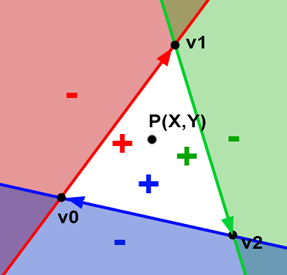
\includegraphics{lit_review/images/EdgeFunctionTriangle.png}
    \caption{Caption\cite{ScratchPixelRasterStage}}
    \label{fig:edgeFunctionTriangle}
\end{figure}

$E_{ab}$ in \Cref{eqn:generalEdgeFunction} is calculated for a point $p$ and can be used to test on which side of a vector $vb-va$ it lies.
\begin{equation}\label{eqn:generalEdgeFunction}
    E_{ab}(x_p, y_p)=(x_p - x_{va})*(y_{vb}-y_{va})-(y_p-y_{va})*(x_{vb}-x_{va}).
\end{equation}
Where $x_n$ is the x coordinate for point $n$ and $y_n$ is the $y$ coordinate for point $n$. 
There are three possible outcomes for this calculation:
\begin{itemize}
    \item $E_{ab}(x_p, y_p) > 0$ if $p$ is on the right of the line
    \item $E_{ab}(x_p, y_p) = 0$ if $p$ is exatly on the line
    \item $E_{ab}(x_p, y_p) < 0$ if $p$ is on the left of the line
\end{itemize}

To test if a given point in inside a triangle all we need to do is calculate the edge functions for each side of the triangle and if the result of each calculation is positive then the point lies in the triangle, this is visualised by \Cref{fig:edgeFunctionTriangle}. 
For a triangle with vertices $v0, v1, v2$ the edge functions in \Cref{eqn:triangleEdgeFunction01},
\Cref{eqn:triangleEdgeFunction12},  \Cref{eqn:triangleEdgeFunction20} are constructed:
\begin{equation}\label{eqn:triangleEdgeFunction01}
    E_{01}(x_p, y_p)=(x_p - x_{v0})*(y_{v1}-y_{v0})-(y_p-y_{v0})*(x_{v1} - x_{v0}) 
\end{equation}
\begin{equation}\label{eqn:triangleEdgeFunction12}
    E_{12}(x_p, y_p)=(x_p - x_{v1})*(y_{v2}-y_{v1})-(y_p-y_{v1})*(x_{v2} - x_{v1}) 
\end{equation}
\begin{equation}\label{eqn:triangleEdgeFunction20}
    E_{20}(x_p, y_p)=(x_p - x_{v2})*(y_{v0}-y_{v2})-(y_p-y_{v2})*(x_{v0} - x_{v2}) 
\end{equation}

The condition for the point lying inside the triangle is therefore shown by \Cref{algorithm:pointInsideTriangleConditionPartial}.

\begin{algorithm}
\caption{An algorithm with caption}\label{algorithm:pointInsideTriangleConditionPartial}
\begin{algorithmic}
    \If{winding order == clockwise}
        \If{$(E_{01}(x_p, y_p) > 0) \; \& \; (E_{12}(x_p, y_p) > 0) \; \& \; (E_{20}(x_p, y_p) > 0)$} 
            \State The point lies inside the triangle.
        \EndIf
    \EndIf
\end{algorithmic}
\end{algorithm}
%https://www.scratchapixel.com/lessons/3d-basic-rendering/rasterization-practical-implementation/rasterization-stage

One thing that is very important to consider is the winding order of the points of the triangle, this will be mentioned in more detail in the future sections. However, the winding order will determine the conditions under which a given point lies in the triangle with reference to the edge functions.

\Cref{fig:edgeFunctionTrianglWinding} shows the difference in the evaluations of the edge functions with with clockwise and counter-clockwise winding order.

\begin{figure}[ht]
    \centering
    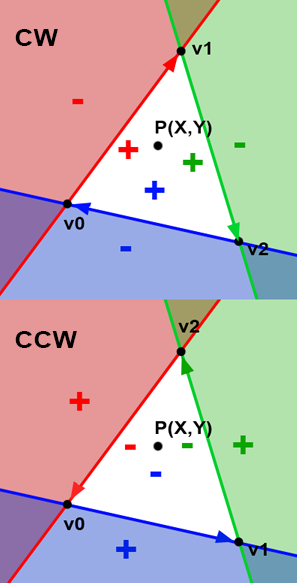
\includegraphics{lit_review/images/EdgeFunctionTriangleWinding.png}
    \caption{Caption\cite{ScratchPixelRasterStage}}
    \label{fig:edgeFunctionTrianglWinding}
\end{figure}

Considering the above we can change the conditions under which the point lies in the triangle to \Cref{algorithm:pointInsideTriangleConditionFull}.

\begin{algorithm}
\caption{An algorithm with caption}\label{algorithm:pointInsideTriangleConditionFull}
\begin{algorithmic}
    \If{winding order == clockwise}
        \If{$(E_{01}(x_p, y_p) > 0) \; \& \; (E_{12}(x_p, y_p) > 0) \; \& \; (E_{20}(x_p, y_p) > 0)$} 
            \State The point lies inside the triangle.
        \EndIf
    \EndIf
    \If{winding order == anti-clockwise}
        \If{$(E_{01}(x_p, y_p) < 0) \; \& \; (E_{12}(x_p, y_p) < 0) \; \& \; (E_{20}(x_p, y_p) < 0)$} 
            \State The point lies inside the triangle.
        \EndIf
    \EndIf
\end{algorithmic}
\end{algorithm}

Using this condition, we can select a point in a pixel in screen space and evaluate the edge functions using that to see if the pixel lie in the triangle and so if it should be rasterized.

\subsection{Pixel Traversal Methods}
The inner loop of the rasterzation algorithm involves traversing every pixel in the screen to see if they overlap the triangle. Since all triangles in the scene will be much smaller than the screen itself there is a lot of wasted work being done.
This provides an opportunity for several optimisations of pixel traversal that will be desacribed in the following sections.

\subsubsection{Pixel By Pixel}
Simplest way of doing this is to construct a bounding box around the triangle, with one of the triangle vertices being a corner of the box.
Then go over all the pixels in the bounding box. If the sample point (usually the centre point) of a given pixel is inside the triangle (computed using the edge equations) then it can continue in the pipeline.

\subsubsection{Bounding Boxes}
The simplest optimisation that can be made, and one of the most impactful, is constructing bounding boxes around a triangle projected to screen space and only traversing those pixels inside the box.

\Cref{fig:triangleBoundingBox} shows the bounding box constructed around the triangle where the vertices of the triangle lie on the edges of the box. This bounding box has edges that lie in the middle of some of the pixels shown on the grid. We therefore expand the bounding box to lie on the edges of all the pixels. The bounding box must also lie entirely in the screen, which means that for a triangle that lies partially outside the screen, the bounding box will cut off part of the triangle.

\begin{figure}[ht]
    \centering
    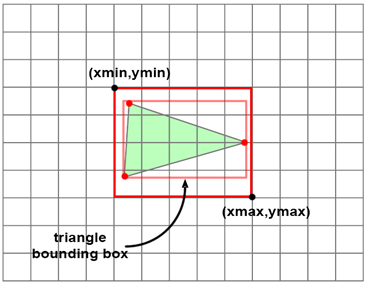
\includegraphics{lit_review/images/triangleBoundingBox.png}
    \caption{from scratch a pixel}
    \label{fig:triangleBoundingBox}
\end{figure}

Given the scale of the bounding box of the triangle in \Cref{fig:triangleBoundingBox}, the bounding box contains 20 pixels. This means that, using this optimization, we have gone from traversing all 2,073,600 pixels in the screen to just traversing 20. 
The only cost to this optimisation is the calculation of the sides of the bounding box, which are few and can be done as in \Cref{algorithm:calculateBoundingBox}.

\begin{algorithm}
\caption{An algorithm with caption}\label{algorithm:calculateBoundingBox}
\begin{algorithmic}


\State $Vertices v0,v1,v2$

//Calculate the floating point bounding box
\State $TopEdge    \gets max(v0.y, v1.y, v2.y)$
\State $BottomEdge \gets min(v0.y, v1.y, v2.y)$
\State $RightEdge  \gets max(v0.x, v1.x, v2.x)$
\State $LeftEdge   \gets min(v0.x, v1.x, v2.x)$

//Expand the bounding box to fit the pixel grid
\State $TopEdge    \gets ciel(TopEdge)$ 

\State $BottomEdge \gets floor(BottomEdge)$
\State $RightEdge  \gets ciel(RightEdge)$
\State $LeftEdge   \gets floor(LeftEdge)$
            
\end{algorithmic}
\end{algorithm}

http://www.sunshine2k.de/coding/java/TriangleRasterization/TriangleRasterization.html

\subsubsection{Scan Line}
\subsubsection{Centre Line}
\subsubsection{Tile Scan}
Another way to do this is to split the bounding box up into tiles. This means fewer operations can be done on tiles which don’t overlap the triangles at all. Tiles which do not lie in the triangle are not evaluated. This method and the Scan line and centre line traversal methods are described by McCormack and McNamara in their paper "Tiled polygon traversal using half-plane edge functions"\cite{McCormackTraversal}. 

\section{Fragment processing}
The rasterizer then produces fragments as output. Fragments are pixel candidates, each pixel can have multiple fragments associated with it. They are produced by the rasterizer. A pixel will have multiple candidates if there are multiple triangles with points on them that map to the same pixel.

The final colour of the pixel will be determined by some combination of these fragments. This can be in the form of a weighted average of the fragment colours for transparent/translucent objects or if the object at the front is opaque then only the closes fragments colour will be used. In the latter case the depth buffer will be enabled allowing for accelerated rendering. 

Fragment shading can also be done as opposed to vertex shading, the difference between these two shading methods can be seen by looking at the difference between Gouraud and Phong shading\cite{gouraudvsphong} which shade the vertices and fragments respectively. 

Because of the interpolation done on the colours of the vertices produced by Gouraud shading, certain artifacts can be produced\cite{gouraudvsphong}.

